\section{Verifying our new features}

To verify that all of the above work as intended, we create a database instance that tests each of these cases, and we verify that the generated web page is correct. Using DB Browser for SQLite \cite{sqliteBrowser}, we populate our data as shown in Figure \ref{fig:db}. Then, by visiting the TestNest page, we can verify a number of items visually in this screenshot of our project's final result, as shown in Figure \ref{fig:site}. Observe that:

\begin{enumerate}
  \item The template displays correctly.
  \item The template inserts the \code{basicpage} widget correctly.
  \item The dynamic route handles complex, nested URIs correctly.
  \item The menu code processes the database instance correctly, including edge cases, i.e. pages where the path, menu title, or menu order is null are not shown in the site's menu.
\end{enumerate}

\begin{figure}[h]
  \centering
  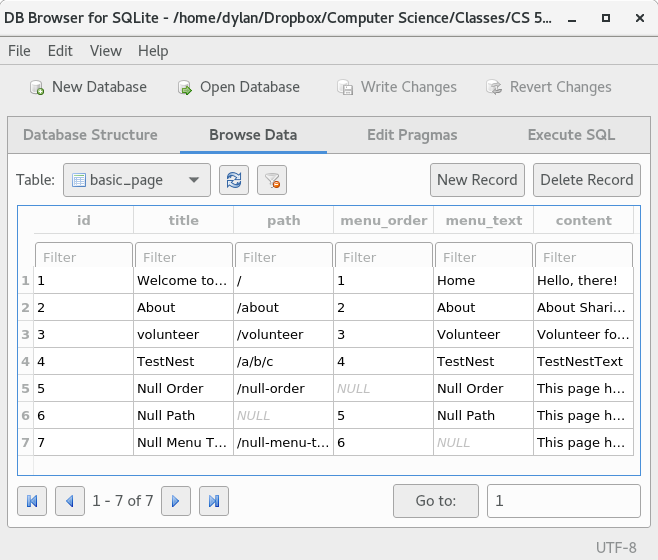
\includegraphics[width=4.4in]{db.png}
  \caption{Our database test instance.}
  \label{fig:db}
\end{figure}

\begin{figure}[h]
  \centering
  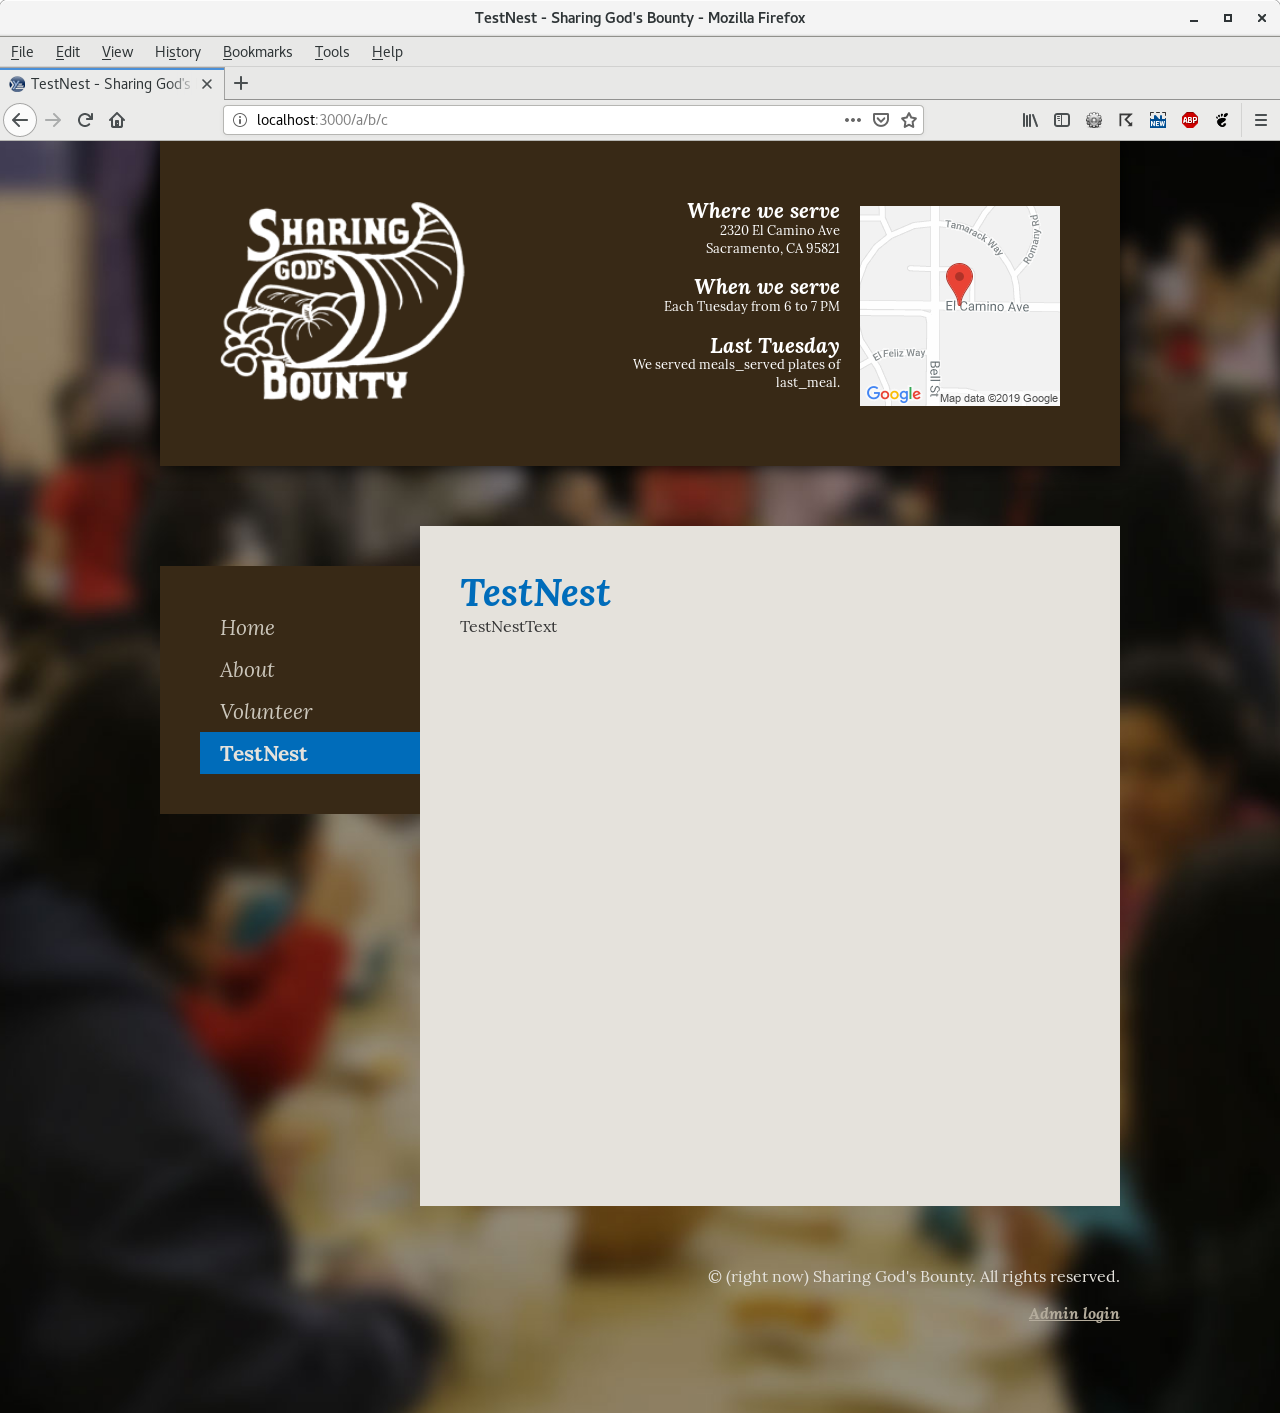
\includegraphics[width=\linewidth]{site.png}
  \caption{Our final website.}
  \label{fig:site}
\end{figure}

\emph{Note: I've tested these features a great deal by clicking through the various pages and hand-checking each attribute as I change it. I sum up all of these checks in this one, informative screenshot to save time, space, and ink.}

\clearpage
